\chapter{Le groupe \mbx{}}
% TODO relecture
	\section{L'historique}
	\begin{description}
		\item[1994] : Création de \memobox{}\\
			\`A l'origine de \memobox{}, deux spécialistes, l'un des services de télécommunications: Christophe \bsc{Fornès} et l'autre du service réseaux: Denis \bsc{Mallet}.\\
			Ensemble, ils décident en 1994 de développer et commercialiser leur propre ligne d'interfaces de communication pour PBX: EdelBox.\\
			Ces interfaces sont commercialisées auprès des éditeurs de logiciels de taxation et d'analyse de trafic téléphonique.

			\memobox{} est né et ne compte aucun salarié.
		
		\item[1995] : Développement commercial\\
			Poussé par ses premiers clients, \memobox{} étend sa gamme en créant un système de taxation téléphonique autonome pour les TPE\footnote{Très Petites Entreprises} et PME\footnote{Petites et Moyennes Entreprises} : Taxabox, décliné également en version hôtelière (Hotelbox).
			Pour se faire, l'entreprise embauche son premier salarié pour étendre ses capacités de développement.
			
		\item[1997] : Le pari du service avec \adt{}\\
			\`A cette date, \memobox{} compte 3 salariés. Après le succès rencontré auprès des éditeurs
			de logiciels et intégrateurs en télécoms, \memobox{} pressant le besoin des entreprises en matière de gestion des coûts télécoms et pour s'adapter
			à son marché, décide de lancer \adt{} le premier service de GFT\footnote{Gestion Financière des Télécoms} en mode hébergé. Une augmentation de capital accompagne ce nouvel axe de développement.
			
		\item[2003] : \memobox{} renforce sa position\\
			Le déploiement des 800 premiers sites nationaux du Ministère de l'Intérieur est bouclé en 4 mois
			et le service satisfait pleinement le client. Pour réaliser cette prouesse, \memobox{} a consolidé ses équipes de développement et d'exploitation.  L'effectif est porté à 13 personnes.
			
		\item[2004] : Les deux fondateurs de \memobox{} rachètent la totalité de l'entreprise.\\
			La bonne santé de \memobox{} en 2004 permet à Christophe \bsc{Fornès} et Denis \bsc{Mallet} de racheter à Global Concept la totalité des parts
			que ce dernier détenait dans l'entreprise. La société est désormais filiale à 100\% du groupe TELECOMS FM\footnote{\textit{Facilities Management}} dont Christophe
			\bsc{Fornès} et Denis \bsc{Mallet} sont les deux seuls actionnaires. \adt{} compte maintenant plus de 2500 sites raccordés et représente désormais 91\% du chiffre d'affaire
			de la société.

		\item[2007] : \memobox{} renforce sa stratégie\\
		Forte de sa politique de développement, \memobox{} décide de renforcer sa stratégie :
		\begin{itemize}
			\item En octobre 2007, elle rachète \techno{} à sa maison mère, \bsc{QUESCOM}.
			\item En décembre 2007, elle lève un million d'euros auprès d'\bsc{ALTO} Invest.
		\end{itemize}
	\end{description}
	\section{La mission de \mbx{}}
	\mbx{} est un éditeur de solutions de \bsc{GFT} et de\textit{ Call Accounting.}
	Forts de leur expérience sur le marché, les deux fondateurs de l'entreprise propose à ses clients une gamme complète d’applications, et de services performants et adaptés aux évolutions permanentes du marché des télécoms.
\newpage	
	La société possède un large panel de clientèle : %%%
	\begin{itemize}
		\item Intégrateurs télécoms,
		\item Prestataires de services,
		\item TPE/PME,
		\item Grandes entreprises,
		\item Administrations et organismes publics.
	\end{itemize}

	La volonté de \mbx{} est également d’être à l’écoute des entreprises pour les conseiller et leur proposer les solutions les mieux adaptées à
	leur besoins. Dans cette optique, ils proposent de nombreuses alternatives à leurs clients en terme de gammes\footnote{logiciels pour PME,
	grands comptes, hôtels, hôpitaux} mais aussi en terme de modes d’installation\footnote{appliances, logiciels ou services externalisés}.

	Ils fournissent aussi des prestations d’administration et d’audit de leurs outils pour permettre aux clients de se concentrer sur le
	c\oe{}ur de leur métier et bénéficier de conseils d’experts avisés.
	
	\section{Les produits de l'entreprise}
		\subsection{Les produits de \techno{}}
		\techno{} a développé les gammes de logiciels suivants:
		\begin{description}	
			\item[GeoTaxe ES] Progiciel destiné aux grandes sociétés, comportant une machine hébergée par les clients collectant leurs données pour les mettre à leurs dispositions via leurs infrastructures internet.
			\item[Geotel] Gestion des appels téléphoniques dans les chambres d'hôtel
			\item[Geopital] Gestion des appels téléphoniques en milieu médicalisé
			\item[Geovox] Serveurs vocaux d'entreprise
		\end{description}
		\subsection{Les produits de \memobox{}}
		\memobox{} a développé les gammes de logiciel suivants:
		\begin{description}	
			\item[\adt{}] Application sous forme de service destinés aux grands comptes
			\item[AUDITELbox] Appliance à installer chez le client de petite taille. Il permet la réalisation d'un audit des télécoms en temps réel.
		\end{description}

	\section{Organisation dans la société}
	\subsection{Mon rôle dans la société}
		J'ai intégré l'équipe de développement de \adt{}, en effet, mon sujet de stage était de refondre le système multi-langues de \adt{}. L'équipe de développement du projet était composée de \Romain{} et de \Denis{}, je me suis rapidement intégré
à l'équipe et ai apporté ma contribution au projet.

\newpage
	\subsection{Le personnel du groupe de Toulouse}
	\begin{description}
		\item[\Denis{}] Vice-président et Directeur Technique
		\item[Jean-Marie \bsc{Lagarde}] Responsable R\&D
		\item[Philippe \bsc{Dureux}] Ingénieur télécoms
		\item[\Romain{}] Ingénieur développement Web
		\item[Mathieu \bsc{Soum}] Stagiaire dans le développement logiciel
		\item[\Adr{}] Stagiaire dans le développement web
	\end{description}
	L'organigramme est disponible figure \ref{organigramme}.
	\begin{figure}[H]
		\centering
		% Graphic for TeX using PGF
% Title: C:\Documents and Settings\antoine.deroquemaure\Mes documents\rapportStage\rapport\images\1-entreprise\oprganigramme.dia
% Creator: Dia v0.97.2
% CreationDate: Tue May 29 14:23:27 2012
% For: antoine.deroquemaure
% \usepackage{tikz}
% The following commands are not supported in PSTricks at present
% We define them conditionally, so when they are implemented,
% this pgf file will use them.
\ifx\du\undefined
  \newlength{\du}
\fi
\setlength{\du}{15\unitlength}
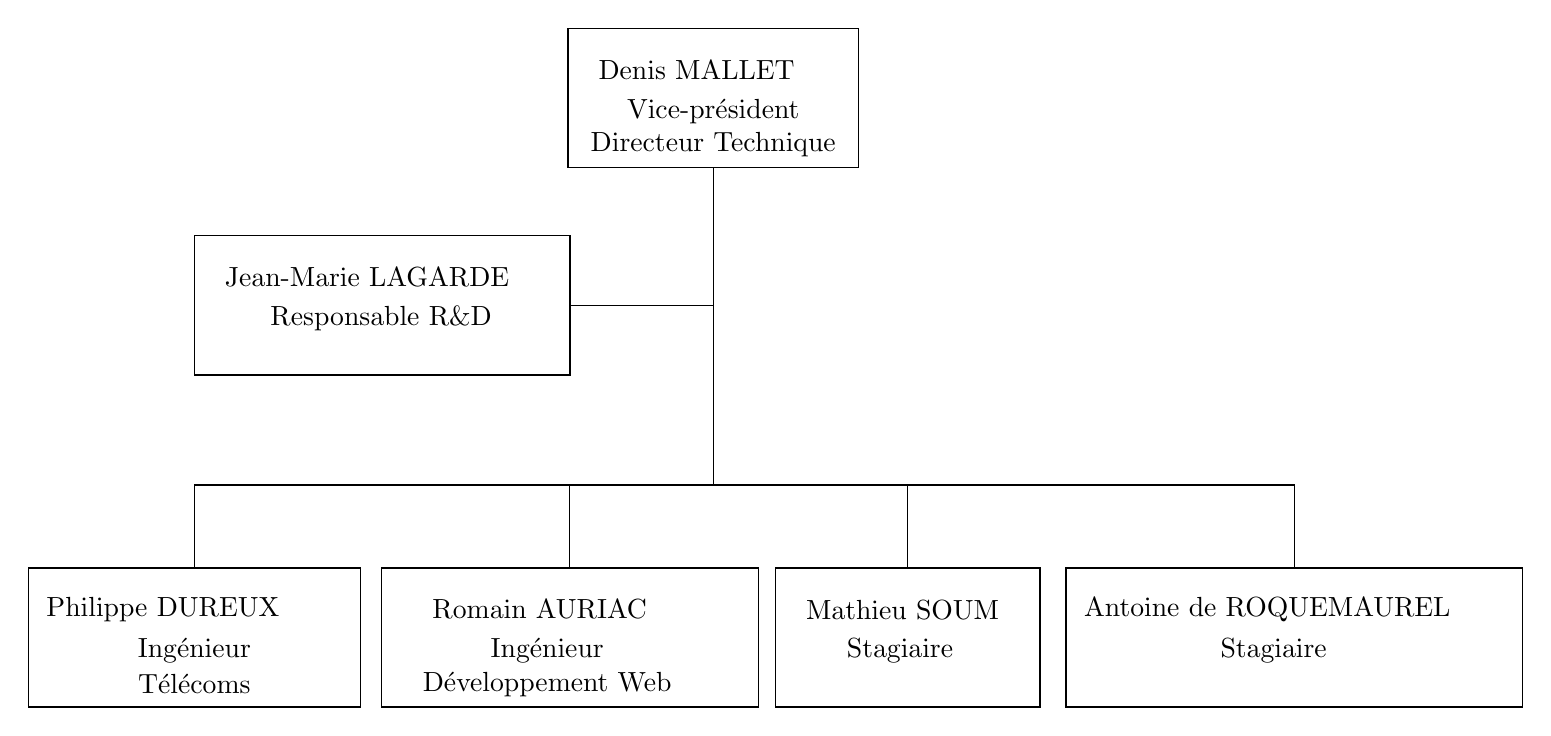
\begin{tikzpicture}
\pgftransformxscale{1.000000}
\pgftransformyscale{-1.000000}
\definecolor{dialinecolor}{rgb}{0.000000, 0.000000, 0.000000}
\pgfsetstrokecolor{dialinecolor}
\definecolor{dialinecolor}{rgb}{1.000000, 1.000000, 1.000000}
\pgfsetfillcolor{dialinecolor}
\pgfsetlinewidth{0.030000\du}
\pgfsetdash{}{0pt}
\pgfsetdash{}{0pt}
\pgfsetmiterjoin
\definecolor{dialinecolor}{rgb}{1.000000, 1.000000, 1.000000}
\pgfsetfillcolor{dialinecolor}
\fill (20.000000\du,-8.000000\du)--(20.000000\du,-4.650000\du)--(27.000000\du,-4.650000\du)--(27.000000\du,-8.000000\du)--cycle;
\definecolor{dialinecolor}{rgb}{0.000000, 0.000000, 0.000000}
\pgfsetstrokecolor{dialinecolor}
\draw (20.000000\du,-8.000000\du)--(20.000000\du,-4.650000\du)--(27.000000\du,-4.650000\du)--(27.000000\du,-8.000000\du)--cycle;
% setfont left to latex
\definecolor{dialinecolor}{rgb}{0.000000, 0.000000, 0.000000}
\pgfsetstrokecolor{dialinecolor}
\node[anchor=west] at (20.500000\du,-7.000000\du){Denis MALLET};
% setfont left to latex
\definecolor{dialinecolor}{rgb}{0.000000, 0.000000, 0.000000}
\pgfsetstrokecolor{dialinecolor}
\node at (23.500000\du,-6.000000\du){Vice-président};
% setfont left to latex
\definecolor{dialinecolor}{rgb}{0.000000, 0.000000, 0.000000}
\pgfsetstrokecolor{dialinecolor}
\node at (23.500000\du,-5.200000\du){Directeur Technique};
\pgfsetlinewidth{0.030000\du}
\pgfsetdash{}{0pt}
\pgfsetdash{}{0pt}
\pgfsetmiterjoin
\definecolor{dialinecolor}{rgb}{1.000000, 1.000000, 1.000000}
\pgfsetfillcolor{dialinecolor}
\fill (7.000000\du,5.000000\du)--(7.000000\du,8.350000\du)--(15.000000\du,8.350000\du)--(15.000000\du,5.000000\du)--cycle;
\definecolor{dialinecolor}{rgb}{0.000000, 0.000000, 0.000000}
\pgfsetstrokecolor{dialinecolor}
\draw (7.000000\du,5.000000\du)--(7.000000\du,8.350000\du)--(15.000000\du,8.350000\du)--(15.000000\du,5.000000\du)--cycle;
% setfont left to latex
\definecolor{dialinecolor}{rgb}{0.000000, 0.000000, 0.000000}
\pgfsetstrokecolor{dialinecolor}
\node[anchor=west] at (7.200000\du,6.000000\du){Philippe DUREUX};
% setfont left to latex
\definecolor{dialinecolor}{rgb}{0.000000, 0.000000, 0.000000}
\pgfsetstrokecolor{dialinecolor}
\node at (11.000000\du,7.000000\du){Ingénieur};
% setfont left to latex
\definecolor{dialinecolor}{rgb}{0.000000, 0.000000, 0.000000}
\pgfsetstrokecolor{dialinecolor}
\node at (11.000000\du,7.800000\du){Télécoms};
\pgfsetlinewidth{0.030000\du}
\pgfsetdash{}{0pt}
\pgfsetdash{}{0pt}
\pgfsetmiterjoin
\definecolor{dialinecolor}{rgb}{1.000000, 1.000000, 1.000000}
\pgfsetfillcolor{dialinecolor}
\fill (15.500000\du,5.000000\du)--(15.500000\du,8.350000\du)--(24.587865\du,8.350000\du)--(24.587865\du,5.000000\du)--cycle;
\definecolor{dialinecolor}{rgb}{0.000000, 0.000000, 0.000000}
\pgfsetstrokecolor{dialinecolor}
\draw (15.500000\du,5.000000\du)--(15.500000\du,8.350000\du)--(24.587865\du,8.350000\du)--(24.587865\du,5.000000\du)--cycle;
% setfont left to latex
\definecolor{dialinecolor}{rgb}{0.000000, 0.000000, 0.000000}
\pgfsetstrokecolor{dialinecolor}
\node[anchor=west] at (16.500000\du,6.000000\du){Romain AURIAC};
% setfont left to latex
\definecolor{dialinecolor}{rgb}{0.000000, 0.000000, 0.000000}
\pgfsetstrokecolor{dialinecolor}
\node at (19.500000\du,7.000000\du){Ingénieur};
% setfont left to latex
\definecolor{dialinecolor}{rgb}{0.000000, 0.000000, 0.000000}
\pgfsetstrokecolor{dialinecolor}
\node at (19.500000\du,7.800000\du){Développement Web};
\pgfsetlinewidth{0.030000\du}
\pgfsetdash{}{0pt}
\pgfsetdash{}{0pt}
\pgfsetmiterjoin
\definecolor{dialinecolor}{rgb}{1.000000, 1.000000, 1.000000}
\pgfsetfillcolor{dialinecolor}
\fill (25.000000\du,5.000000\du)--(25.000000\du,8.350000\du)--(31.371733\du,8.350000\du)--(31.371733\du,5.000000\du)--cycle;
\definecolor{dialinecolor}{rgb}{0.000000, 0.000000, 0.000000}
\pgfsetstrokecolor{dialinecolor}
\draw (25.000000\du,5.000000\du)--(25.000000\du,8.350000\du)--(31.371733\du,8.350000\du)--(31.371733\du,5.000000\du)--cycle;
% setfont left to latex
\definecolor{dialinecolor}{rgb}{0.000000, 0.000000, 0.000000}
\pgfsetstrokecolor{dialinecolor}
\node[anchor=west] at (25.500000\du,6.000000\du){Mathieu SOUM};
% setfont left to latex
\definecolor{dialinecolor}{rgb}{0.000000, 0.000000, 0.000000}
\pgfsetstrokecolor{dialinecolor}
\node at (28.000000\du,7.000000\du){Stagiaire};
\pgfsetlinewidth{0.030000\du}
\pgfsetdash{}{0pt}
\pgfsetdash{}{0pt}
\pgfsetmiterjoin
\definecolor{dialinecolor}{rgb}{1.000000, 1.000000, 1.000000}
\pgfsetfillcolor{dialinecolor}
\fill (32.000000\du,5.000000\du)--(32.000000\du,8.350000\du)--(43.000000\du,8.350000\du)--(43.000000\du,5.000000\du)--cycle;
\definecolor{dialinecolor}{rgb}{0.000000, 0.000000, 0.000000}
\pgfsetstrokecolor{dialinecolor}
\draw (32.000000\du,5.000000\du)--(32.000000\du,8.350000\du)--(43.000000\du,8.350000\du)--(43.000000\du,5.000000\du)--cycle;
% setfont left to latex
\definecolor{dialinecolor}{rgb}{0.000000, 0.000000, 0.000000}
\pgfsetstrokecolor{dialinecolor}
\node[anchor=west] at (32.200000\du,6.000000\du){Antoine de ROQUEMAUREL};
% setfont left to latex
\definecolor{dialinecolor}{rgb}{0.000000, 0.000000, 0.000000}
\pgfsetstrokecolor{dialinecolor}
\node at (37.000000\du,7.000000\du){Stagiaire};
% setfont left to latex
\definecolor{dialinecolor}{rgb}{0.000000, 0.000000, 0.000000}
\pgfsetstrokecolor{dialinecolor}
\node at (37.000000\du,7.800000\du){};
\pgfsetlinewidth{0.030000\du}
\pgfsetdash{}{0pt}
\pgfsetdash{}{0pt}
\pgfsetmiterjoin
\definecolor{dialinecolor}{rgb}{1.000000, 1.000000, 1.000000}
\pgfsetfillcolor{dialinecolor}
\fill (11.000000\du,-3.000000\du)--(11.000000\du,0.350000\du)--(20.050000\du,0.350000\du)--(20.050000\du,-3.000000\du)--cycle;
\definecolor{dialinecolor}{rgb}{0.000000, 0.000000, 0.000000}
\pgfsetstrokecolor{dialinecolor}
\draw (11.000000\du,-3.000000\du)--(11.000000\du,0.350000\du)--(20.050000\du,0.350000\du)--(20.050000\du,-3.000000\du)--cycle;
% setfont left to latex
\definecolor{dialinecolor}{rgb}{0.000000, 0.000000, 0.000000}
\pgfsetstrokecolor{dialinecolor}
\node[anchor=west] at (11.500000\du,-2.000000\du){Jean-Marie LAGARDE};
% setfont left to latex
\definecolor{dialinecolor}{rgb}{0.000000, 0.000000, 0.000000}
\pgfsetstrokecolor{dialinecolor}
\node at (15.500000\du,-1.000000\du){Responsable R\&D};
\pgfsetlinewidth{0.030000\du}
\pgfsetdash{}{0pt}
\pgfsetdash{}{0pt}
\pgfsetmiterjoin
\pgfsetbuttcap
{
\definecolor{dialinecolor}{rgb}{0.000000, 0.000000, 0.000000}
\pgfsetfillcolor{dialinecolor}
% was here!!!
{\pgfsetcornersarced{\pgfpoint{0.000000\du}{0.000000\du}}\definecolor{dialinecolor}{rgb}{0.000000, 0.000000, 0.000000}
\pgfsetstrokecolor{dialinecolor}
\draw (23.500000\du,-4.650000\du)--(23.500000\du,3.000000\du)--(28.185867\du,3.000000\du)--(28.185867\du,4.986438\du);
}}
\pgfsetlinewidth{0.030000\du}
\pgfsetdash{}{0pt}
\pgfsetdash{}{0pt}
\pgfsetmiterjoin
\pgfsetbuttcap
{
\definecolor{dialinecolor}{rgb}{0.000000, 0.000000, 0.000000}
\pgfsetfillcolor{dialinecolor}
% was here!!!
{\pgfsetcornersarced{\pgfpoint{0.000000\du}{0.000000\du}}\definecolor{dialinecolor}{rgb}{0.000000, 0.000000, 0.000000}
\pgfsetstrokecolor{dialinecolor}
\draw (23.500000\du,-4.650000\du)--(23.500000\du,3.000000\du)--(11.000000\du,3.000000\du)--(11.000000\du,5.000000\du);
}}
\pgfsetlinewidth{0.030000\du}
\pgfsetdash{}{0pt}
\pgfsetdash{}{0pt}
\pgfsetmiterjoin
\pgfsetbuttcap
{
\definecolor{dialinecolor}{rgb}{0.000000, 0.000000, 0.000000}
\pgfsetfillcolor{dialinecolor}
% was here!!!
{\pgfsetcornersarced{\pgfpoint{0.000000\du}{0.000000\du}}\definecolor{dialinecolor}{rgb}{0.000000, 0.000000, 0.000000}
\pgfsetstrokecolor{dialinecolor}
\draw (23.500000\du,-4.650000\du)--(23.500000\du,3.000000\du)--(20.043932\du,3.000000\du)--(20.043932\du,5.000000\du);
}}
\pgfsetlinewidth{0.030000\du}
\pgfsetdash{}{0pt}
\pgfsetdash{}{0pt}
\pgfsetmiterjoin
\pgfsetbuttcap
{
\definecolor{dialinecolor}{rgb}{0.000000, 0.000000, 0.000000}
\pgfsetfillcolor{dialinecolor}
% was here!!!
{\pgfsetcornersarced{\pgfpoint{0.000000\du}{0.000000\du}}\definecolor{dialinecolor}{rgb}{0.000000, 0.000000, 0.000000}
\pgfsetstrokecolor{dialinecolor}
\draw (23.500000\du,-4.650000\du)--(23.500000\du,3.000000\du)--(37.500000\du,3.000000\du)--(37.500000\du,5.000000\du);
}}
\pgfsetlinewidth{0.030000\du}
\pgfsetdash{}{0pt}
\pgfsetdash{}{0pt}
\pgfsetmiterjoin
\pgfsetbuttcap
{
\definecolor{dialinecolor}{rgb}{0.000000, 0.000000, 0.000000}
\pgfsetfillcolor{dialinecolor}
% was here!!!
{\pgfsetcornersarced{\pgfpoint{0.000000\du}{0.000000\du}}\definecolor{dialinecolor}{rgb}{0.000000, 0.000000, 0.000000}
\pgfsetstrokecolor{dialinecolor}
\draw (23.500000\du,-4.650000\du)--(23.500000\du,-1.325000\du)--(20.050000\du,-1.325000\du);
}}
\end{tikzpicture}


		\caption{Organigramme du service R\&D à Toulouse}
		\label{organigramme}
	\end{figure}

	\subsection{Les horaires de travail}
        Les horaires de l'entreprise sont assez souples, cependant afin d'assurer un standard téléphonique, tous les employés doivent être présents entre 9h30 et 17h30.

        Pour ma part, j'arrivais le matin vers 9h30, allais déjeuner vers 12h30 et reprenais le travail de 14h jusqu'à 18h30.
	\section{L'environnement de travail}
    \subsection{Mon poste de travail}
        Je travaillais sous un environnement Windows XP Professionnel SP3, ce système était installé sur un ordinateur de série Dell, munit d'un processeur Intel Core 2 Duo cadencé à 2Ghz avec 2Gio de RAM.

        Ce poste possédait deux écrans, ainsi je pouvais travailler plus vite en ayant des applications réparties sur les deux écrans.
	\subsection{Le serveur web}
		Afin de pouvoir effectuer des tests, j'utilisais un serveur distant, situé dans les locaux de l'entreprise.
		Ce serveur, nommé \texttt{to-audidev-mbx} était un serveur FreeBSD, avec un serveur Apache et une base de données MySQL.
		Ce serveur n'était destiné qu'au développement, ainsi nous avions une base de données permettant les tests éventuels. Une fois que des
		modifications stables ont été effectuées et commitées, celles-ci étaient basculées en production, sur un serveur situé à Paris.
	\subsection{Pour le développement}
		J'ai utilisé l'environnement de Développement Intégré\footnote{EDI} Eclipse, il a l'avantage d'être gratuit et très modulable; grâce aux nombreux
		projets qui ont été réalisés pour cette plateforme. Dans l'entreprise tout le monde l'utilisait, que ce soit pour du PHP ou du C++. En
		ce qui me concerne, j'avais un environnement PHP, je possédais le projet \textit{PHP Development Tools}\footnote{PDT}. Il
		permet de faire de l'analyse syntaxique, de l'autocomplétion ainsi que la navigation entre les classes et méthodes.
	\subsection{Pour le travail collaboratif}
		N'étant pas seul sur le projet, il a fallu mettre en place des outils permettant le travail collaboratif. Pour cela tous les projets
		de la société sont regroupés sous un système de gestion de versions, en l'occurrence, SubVersioN. Ce système permet d'enregistrer toutes les modifications
		effectuées sur un fichier. Ainsi chaque collaborateur peut mettre à jour, comparer ou récupérer une ancienne version d'un fichier.
		Pour avoir un environnement Eclipse complet, il y a été rajouté le projet \textit{subclipse} proposé par Tigris.org. Il contient svnClientAdapter
		et SVNKit.
	\subsection{Pour la synchronisation serveur}
		Le site de développement étant sur un serveur distant, il fallait pouvoir synchroniser mes modifications avec ce serveur, ainsi tous les développeurs web utilisaient un plugin eclipse appelé FileSync qui synchronisait nos fichiers avec le serveur à chaque enregistrement du fichier.
